
\section{enzymes.xml}

The enzyme file is used to define enzyme composition and efficiency.

\subsection{RBAEnzymes}
\label{sec:rba_enzymes}

The outermost portion of the metabolism file is an instance of class
\rbaenzymes, shown in Figure~\ref{fig:enzymes_doc}.

\begin{figure}
  \centering
  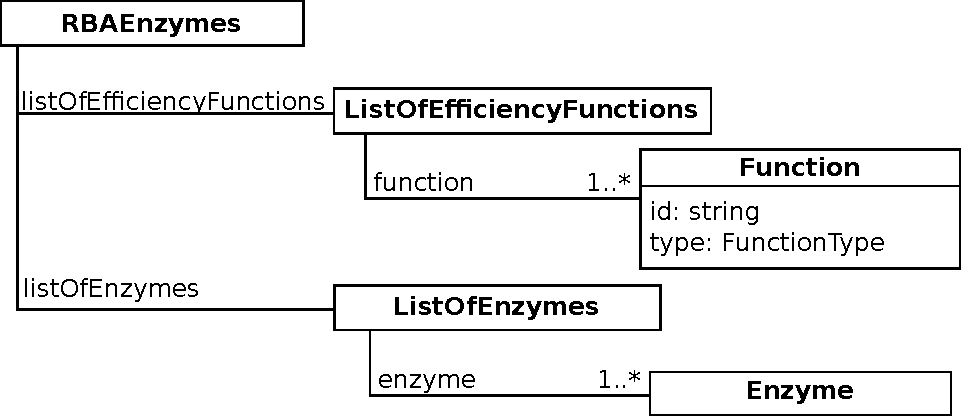
\includegraphics[scale=0.8]{figures/enzymes_doc}
  \caption{XML structure of enzyme document.}
\label{fig:enzymes_doc}
\end{figure}

\rbaenzymes{} has no simple attributes.
It contains exactly one instance of \textbf{ListOfEfficiencyFunctions}.

It contains excatly one instance of \textbf{ListOfEnzymes}.


\subsection{Enzyme}
\label{sec:enzyme}

The \enzyme{} class is used to define enzymes
(Fig.~\ref{fig:enzymes_enzyme}).

\begin{figure}
  \centering
  \includegraphics[scale=0.8]{figures/enzymes_enzyme}
  \caption{Class storing enzyme information.}
\label{fig:enzymes_enzyme}
\end{figure}

Its composition is given by a \textbf{ListOfComponentReferences}.

\paragraph{The \textit{id} attribute}
The \textbf{id} attribute is a string defining the identifier of
the macromolecule.

\paragraph{The \textit{compartment} attribute}
The \textbf{compartment} attribute must match the identifier of a \compartment.
It represents the compartment where the molecule is thought to be active.


\subsection{EnzymeEfficiency}
\label{sec:enzyme_efficiency}

The \enzymeefficiency{} class is used to (Fig.~\ref{fig:enzymes_enzyme}).

\paragraph{The \textit{function} attribute}
The \textbf{function} attribute must match the identifier of a \component{}
defined in the same \rbamacromolecules{} instance.
